\part{�tude 2: encodage de l'intention et de l'ex�cution motrice}
\label{Etude2_encodage}

\begin{chapintro}
  \malettrine{C}{e}  chapitre  introductif  gnagnagna.

  Pas obligatoire !

\end{chapintro}

%%% --------------------------
%%% R�sum� de l'article
%%% --------------------------
\section{r�sum� de l'�tude}

%%% --------------------------
%%% Article
%%% --------------------------
\section{article}
%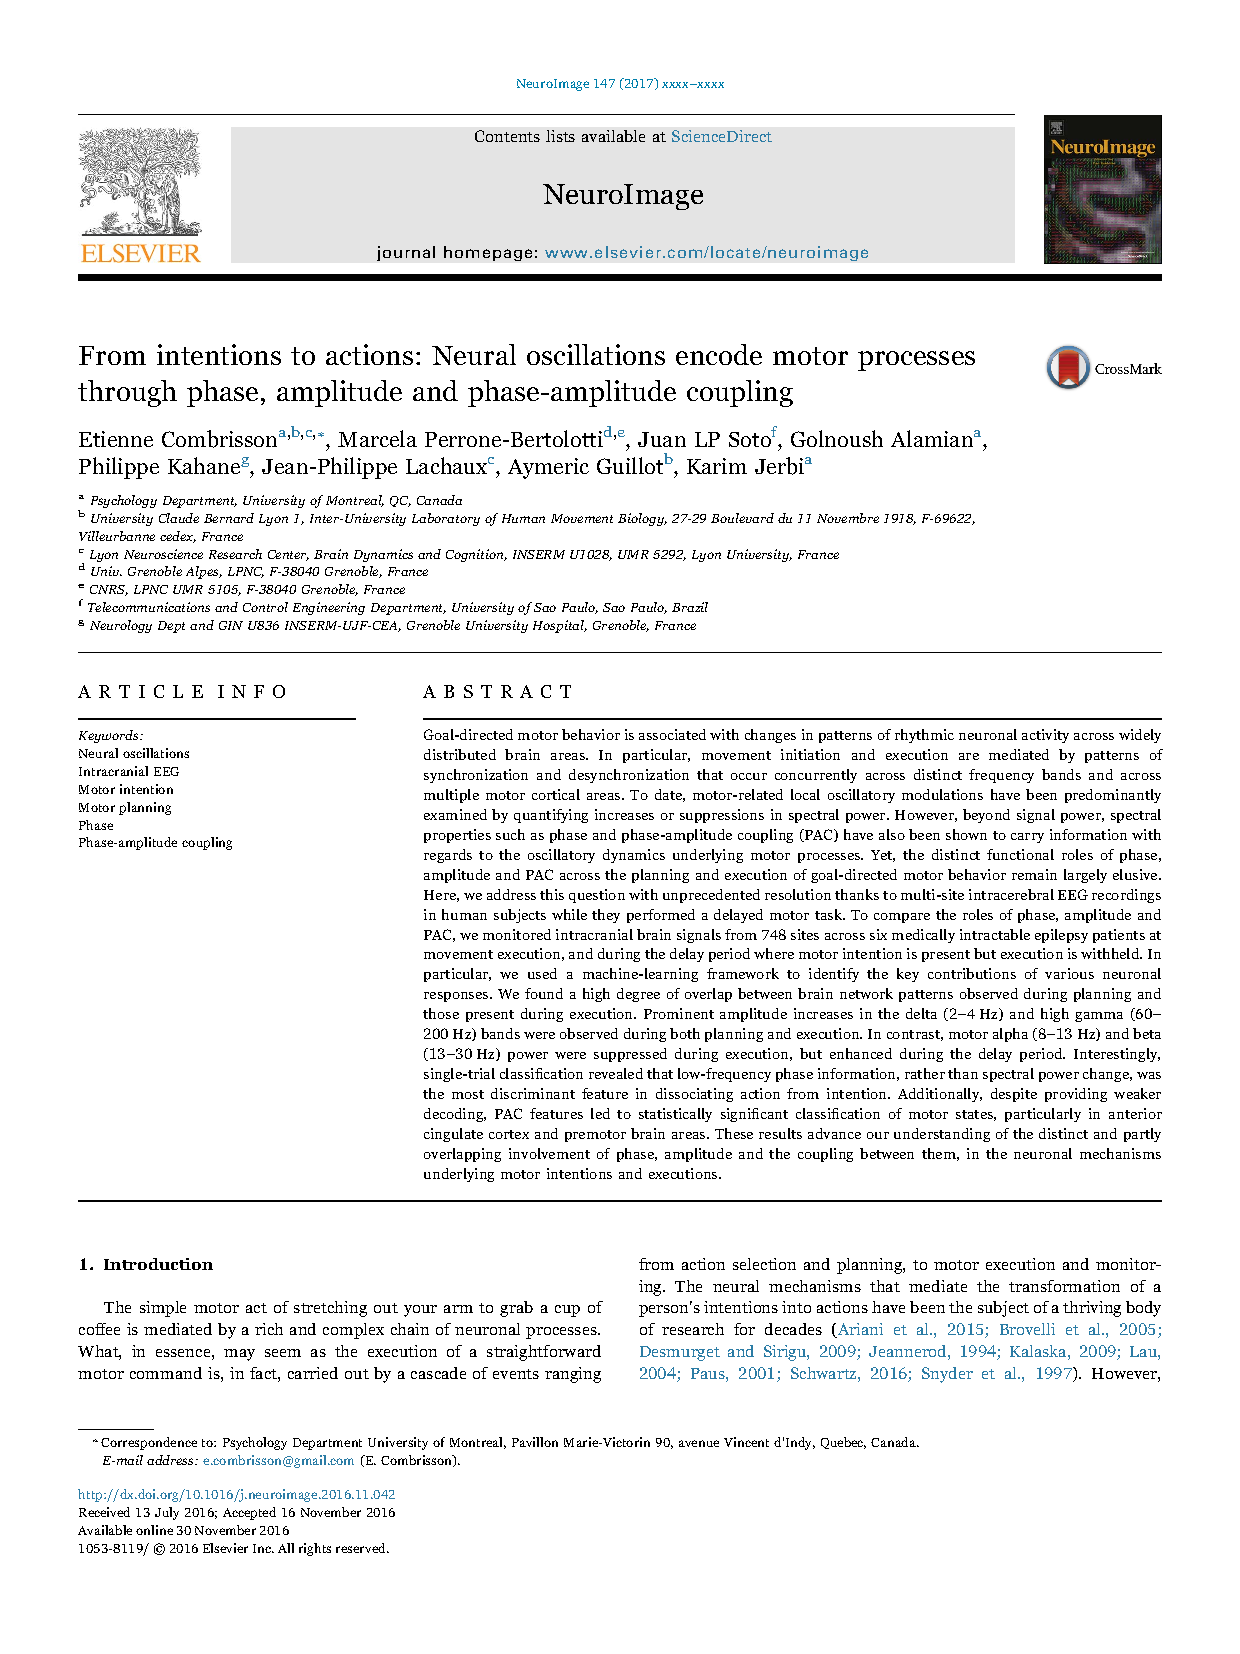
\includepdf[pages={1-29}]{Chap2/Etude2_Combrisson-etal-Encoding-Intention-Execution.pdf}

%%% --------------------------
%%% Conclusion de l'article??
%%% --------------------------
\section*{conclusion du chapitre}
\addcontentsline{toc}{section}{Conclusion}

Ceci est la conclusion. Personnellement, je n'aime pas que la conclusion 
soit num�rot�, mais je veux qu'elle apparaisse dans la table des mati�re, d'o� 
la commande addcontentsline.

